\documentclass[xcolor=table]{beamer}
\usetheme{uic}
\usepackage{minted}
\usepackage{amsfonts,amsmath,oldgerm,algorithmic,algorithm}
\usepackage[font=small,labelfont=bf]{caption} % Required for specifying captions to tables and figures
\usepackage{tcolorbox}
\tcbuselibrary{listings,skins}
\usepackage{alltt,xcolor}
\usepackage{hyperref}
\usepackage{comment}
\usepackage{amsthm}
\usepackage[spanish]{babel}


\lstdefinestyle{mystyle}{
language=C
}

\newtcblisting{mylisting}[2][]{
    arc=0pt, outer arc=0pt,
    listing only, 
    listing style=mystyle,
    title=#2,
    #1
}


\newcommand{\hrefcol}[2]{\textcolor{uihteal}{\href{#1}{#2}}}
\newcommand{\testcolor}[1]{\colorbox{#1}{\textcolor{#1}{test}}~\texttt{#1}}

% Please see Section 18.1 of Beamer User Guide for all the options \usefonttheme provides
\usefonttheme[onlymath]{serif}
% \usefonttheme{serif} % use this if you would like Serif font throughout (and not just for math)

\title{Fundamentos de Inteligencia Artificial}
\titlebackground{images/etsiinformatica3.jpeg}
% an asterisk will split the background:
% \titlebackground*{images/uic_seo.jpg}
\subtitle{Técnicas básicas de optimización}

\author{\href{mailto:jmmontes@uma.es}{José A. Montenegro}}
\date{\today}

%https://aima.cs.berkeley.edu/algorithms.pdf


\begin{document}

\newtheorem{mydef}{Definición}[section] % Añade [section] para que se reinicie en cada sección
\maketitle

% default is no footline, but page numbers are incredibly useful for the audience to ask questions later
\footlinecolor{uicblue}

%%%%%%%%%%%%%%%%%%%%%%%%%%%%%%%%%%%%%%%%%%%%%%%%%%%
%%%%%%%%%%%%%%%%%%%%%%%%%%%%%%%%%%%%%%%%%%%%%%%%%%%
%%%%%%%%%%%%%%%%%%%%%%%%%%%%%%%%%%%%%%%%%%%%%%%%%%%
%%%%%%%%%%%%%%%%%%%%%%%%%%%%%%%%%%%%%%%%%%%%%%%%%%%
%%%%%%%%%%%%%%%%%%%%%%%%%%%%%%%%%%%%%%%%%%%%%%%%%%%
%%%%%%%%%%%%%%%%%%%%%%%%%%%%%%%%%%%%%%%%%%%%%%%%%%%


%%%%%%%%%%%%%%%%%%%%%%%%%%%%%%%%%%%%%%%%%%%%%%%%%%%
%%%%%%%%%%%%%%%%%%%%%%%%%%%%%%%%%%%%%%%%%%%%%%%%%%%
%%%%%%%%%%%%%%%%%%%%%%%%%%%%%%%%%%%%%%%%%%%%%%%%%%%
%%%%%%%%%%%%%%%%%%%%%%%%%%%%%%%%%%%%%%%%%%%%%%%%%%%
%%%%%%%%%%%%%%%%%%%%%%%%%%%%%%%%%%%%%%%%%%%%%%%%%%%
%%%%%%%%%%%%%%%%%%%%%%%%%%%%%%%%%%%%%%%%%%%%%%%%%%%


\begin{frame}{Contenido}
\tableofcontents
\end{frame}

%%%%%%%%%%%%%%%%%%%%%%%%%%%%%%%%
%%%%%%%%%%%%%%%%%%%%%%%%%%%%%%%%
%SECCION %%%%%%%%%%%%%%%%%%%%%%%%%%%%%%%
%%%%%%%%%%%%%%%%%%%%%%%%%%%%%%%%
%%%%%%%%%%%%%%%%%%%%%% 

\begin{chapter}[images/etsiinformatica4.png]{uicblue}{Búsqueda local}
\end{chapter}

%%%%%%%%%%%%%%%%%%%%%%%%%%%%%%%%
%%%%%%%%%%%%%%%%%%%%%%%%%%%%%%%%
%%%%%%%%%%%%%%%%%%%%%%%%%%%%%%%%

%%%%%%%%%%%%%%%%%%%%%%%%%%%%%%%%
%%%%%%%%%%%%%%%%%%%%%%%%%%%%%%%%

%%%%%%%%%%%%%%%%%%%%%%%%%%%%%%%%

\section{Búsqueda Local}
%%%%%%%%%%%%%%%%%%%%%%%%%%%%%%%%
%%%%%%%%%%%%%%%%%%%%%%%%%%%%%%%%

%%%%%%%%%%%%%%%%%%%%%%%%%%%%%%%%

\begin{frame} \frametitle{Búsqueda Local} \small

\begin{itemize}
\item Los algoritmos anteriores exploran los espacios de búsqueda y la solución a los problemas son el camino desde el origen al objetivo.
\begin{itemize}
\item Existen problemas donde el camino al objetivo es irrelevante.
\end{itemize}
\item Búsqueda local son algoritmos útiles para resolver problemas de optimización, encontrar el mejor estado según función objetivo.
\item El espacio de búsqueda está formado por estados, que vienen dados por el valor de una  función objetivo, que puede ser maximizar o minimizar.
\end{itemize}

\end{frame} 
%%%%%%%%%%%%%%%%%%%%%%%%%%%%%%%%

\begin{frame} \frametitle{Búsqueda Local} \small

\begin{figure}
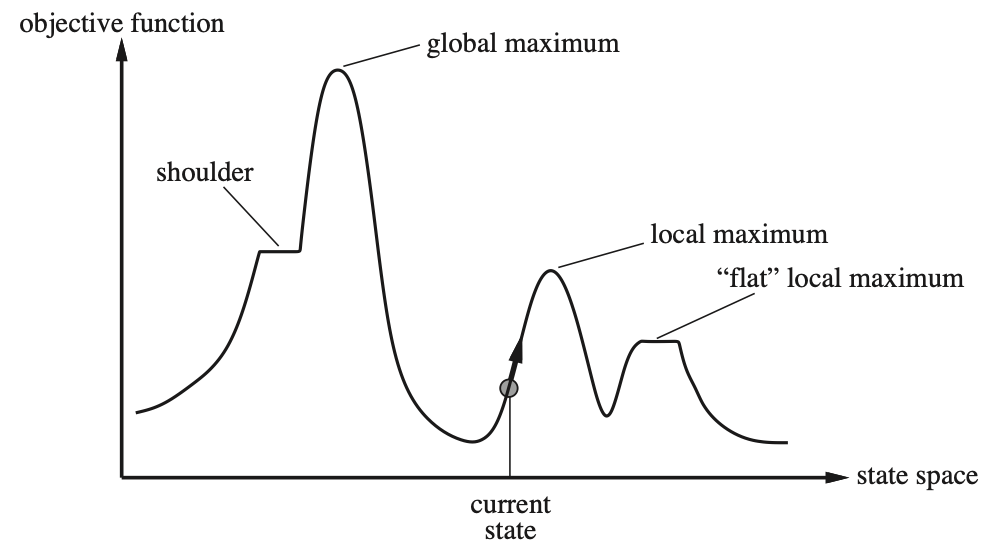
\includegraphics[scale=0.55]{./img/BusquedaLocal}
\end{figure}


\end{frame} 


\begin{chapter}[images/etsiinformatica4.png]{uicblue}{Búsqueda local\\
Hill Climbing}
\end{chapter}
\subsection{Hill Climbing}
%%%%%%%%%%%%%%%%%%%%%%%%%%%%%%%%
%%%%%%%%%%%%%%%%%%%%%%%%%%%%%%%%

%%%%%%%%%%%%%%%%%%%%%%%%%%%%%%%%

\begin{frame} \frametitle{Hill Climbing} \small

\begin{itemize}
\item El algoritmo se mueve continuamente en dirección del valor creciente (maximizar), es decir, cuesta arriba.
\item Finaliza cuando alcanza ``un pico'' donde ningún vecino tiene un valor más alto (maximizar).
\item El algoritmo no mantiene un árbol de búsqueda, solo nodo actual y valor función objetivo.
\item Similar a Greedy en que utiliza sólo la heurística, pero no busca eun camino distinto, ya que no tiene memoria de donde ha estado.
\end{itemize}

\end{frame} 


%%%%%%%%%%%%%%%%%%%%%%%%%%%%%%%%

\begin{frame} \frametitle{Hill Climbing} \small

\begin{figure}
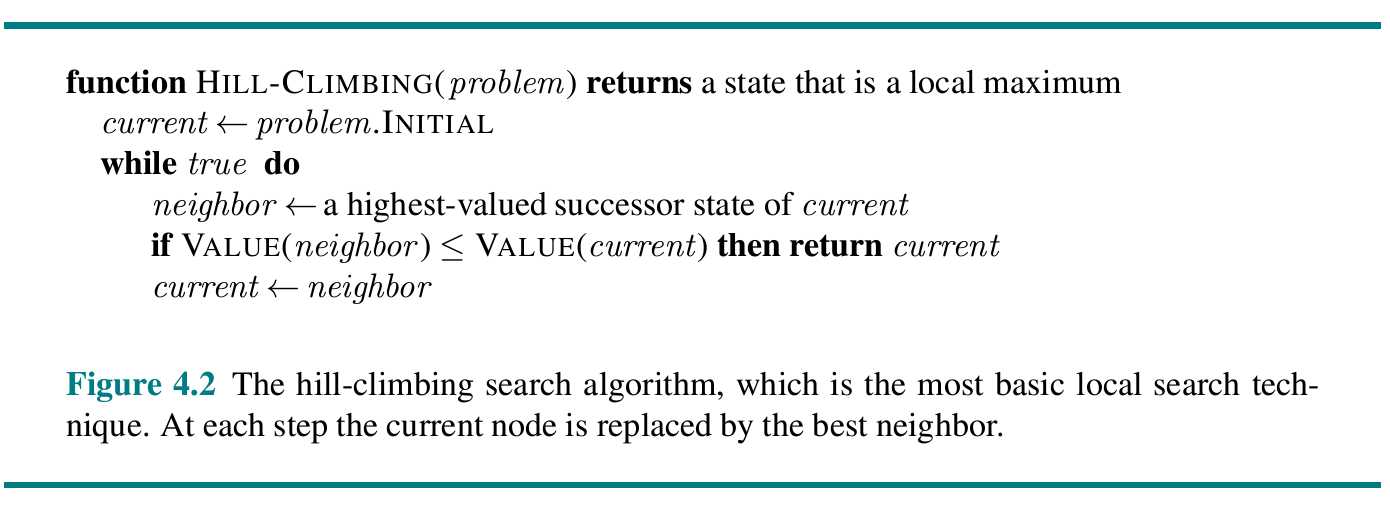
\includegraphics[scale=0.45]{./img/AlgoritmoHC}
\end{figure}


\end{frame} 

%%%%%%%%%%%%%%%%%%%%%%%%%%%%%%%%
\begin{frame} [fragile ]\frametitle{Hill Climbing (Minimizar) en Python } \footnotesize
\begin{minted}[fontsize=\tiny]{python}

def hill_climbing(problem, max_iterations=1000):
    current_state = problem.state
    current_cost = problem.calculate_cost(current_state)
    print ("current_cost:", current_cost)

    for _ in range(max_iterations):
        neighbors = problem.get_neighbors()
        print ("\t neighbors:", neighbors)

        best_neighbor       = min(neighbors, key=lambda state: problem.calculate_cost(state))
        best_neighbor_cost  = problem.calculate_cost(best_neighbor)
        print ("\t\t best_neighbor:", best_neighbor," - ",best_neighbor_cost)

        if best_neighbor_cost >= current_cost: 
            return current_state
        
        problem.state = best_neighbor
        current_state = best_neighbor
        current_cost = best_neighbor_cost

\end{minted}

\end{frame} 

%%%%%%%%%%%%%%%%%%%%%%%%%%%%%%%%

\begin{frame} \frametitle{Hill Climbing - Puzzle 8} \small

\begin{figure}
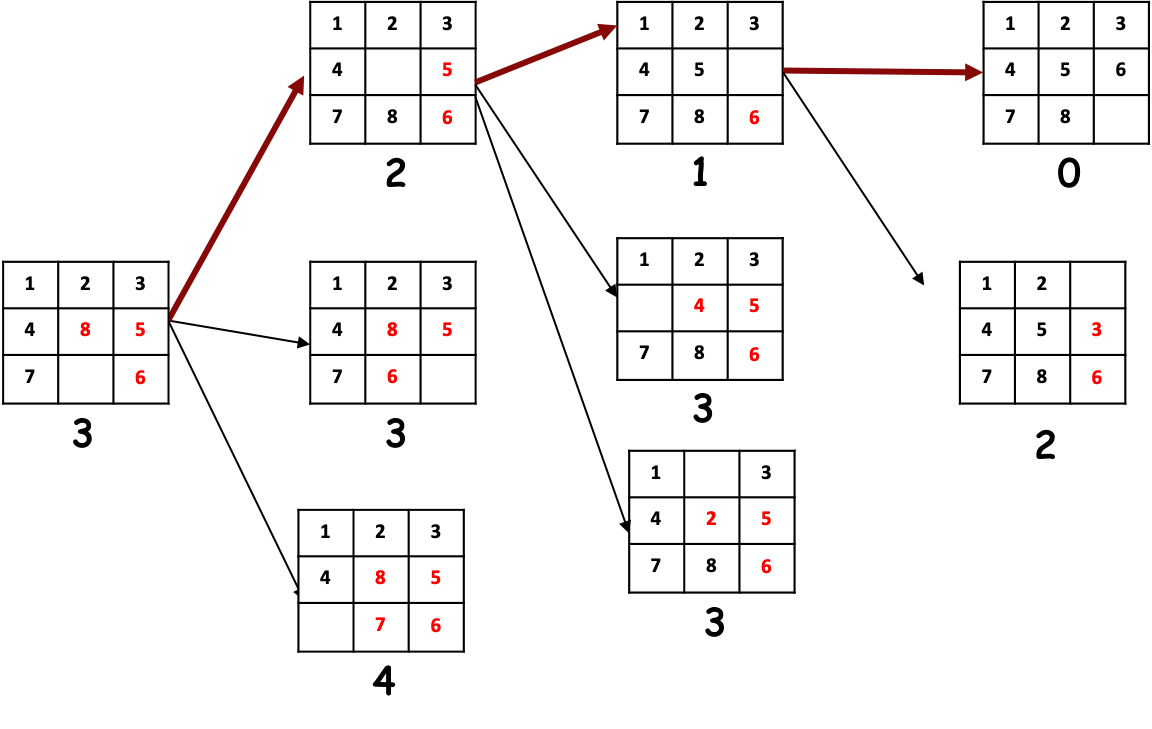
\includegraphics[scale=0.45]{./img/Puzzle8HC}
\end{figure}


\end{frame} 


%%%%%%%%%%%%%%%%%%%%%%%%%%%%%%%%

\begin{frame} \frametitle{Hill Climbing - Problemas Hill Climbing} \small

\begin{itemize}
\item \textbf{Máximo Local}: El valor no es el punto más elevado en el espacio de estados.
\item \textbf{Meseta}: El espacio tiene una región plana, que si coincide con un máximo local no hay solución posible.
\item \textbf{Remedio}: Comienzos estado aleatorio.
\end{itemize}



\begin{figure}
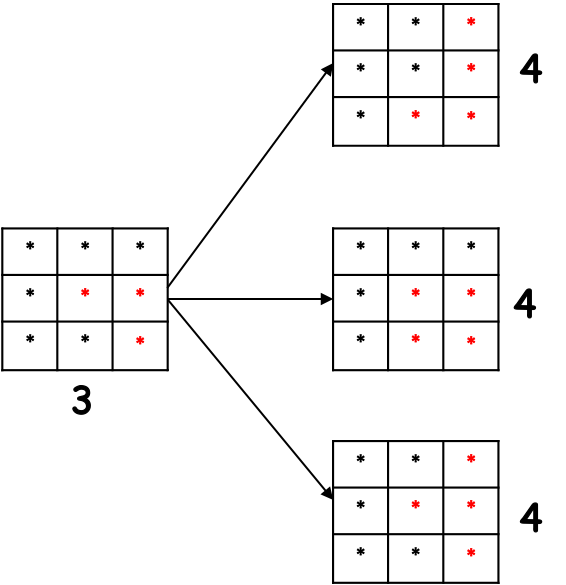
\includegraphics[scale=0.35]{./img/ProblemasHC}
\end{figure}


\end{frame} 

%%%%%%%%%%%%%%%%%%%%%%%%%%%%%%%%

\begin{frame} \frametitle{ Ejemplo 8 Reinas} \tiny

\begin{itemize}
\item El objetivo del problema es establecer 8 reinas en un tablero de forma que no se ataquen entre sí. 
\item Evitar Misma fila, columna o diagonal.
\end{itemize}

\begin{description}
\item[Estado] : Cualquier representación de 8 reinas en el tablero.
\item[Estado Inicial] : Tablero con 8 reinas
\item[Acciones] : Mover una reina a una casilla vacía de una columna
\item[Modelo Transición] : Devuelve tablero con una reina añadida en una casilla determinada.
\item[Test Objetivo] : 8 reinas en el tablero que no se ataquen entre sí.
\item[Función Heurística] : Número de pares de reinas que se atacan (MIN) 
\end{description}




\begin{figure}
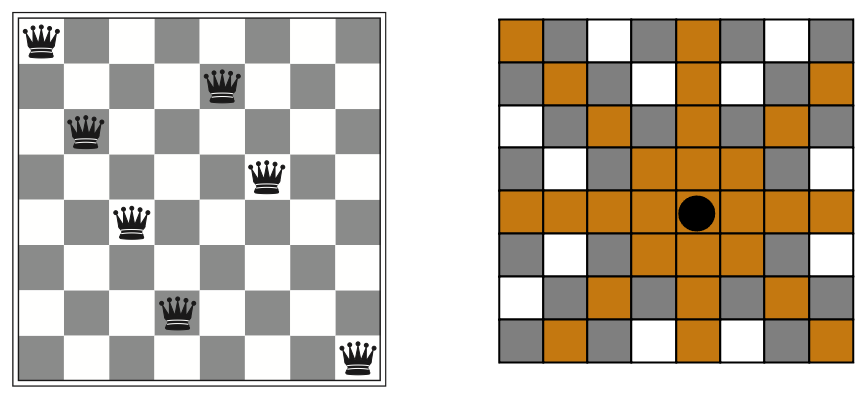
\includegraphics[scale=0.45]{./img/8Reinas}
\end{figure}


\end{frame} 
%%%%%%%%%%%%%%%%%%%%%%%%%%%%%%%%

\begin{frame} \frametitle{ Ejemplo 8 Reinas} \small

\begin{itemize}
\item Los sucesores de un estado son todos los posibles estados generados al mover una reina en una columna (8x7=56 sucesores). 
\item Partiendo de (1) llegamos a (2) en 5 pasos y queda en mínimo local.
\end{itemize}



\begin{figure}
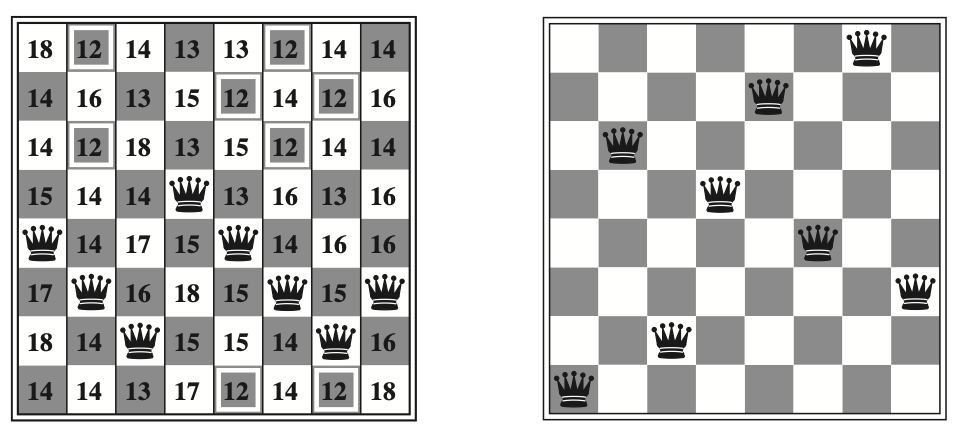
\includegraphics[scale=0.45]{./img/8ReinasHeuristicas}
\end{figure}

\begin{center}
(1) h= 3+4+2+3+2+2+1=17	\hspace{1cm} (2) h=0+0+0+1+0+0+0+0=1
\end{center}

\end{frame} 


%%%%%%%%%%%%%%%%%%%%%%%%%%%%%%%%
%%%%%%%%%%%%%%%%%%%%%%%%%%%%%%%%
\begin{chapter}[images/etsiinformatica4.png]{uicblue}{Búsqueda local\\
Recorrido Simulado}
\end{chapter}
\subsection{Recorrido Simulado}
%%%%%%%%%%%%%%%%%%%%%%%%%%%%%%%%

\begin{frame} \frametitle{ Recorrido Simulado} \small

\begin{itemize}
\item Algoritmo anterior no realiza movimientos ``cuesta abajo'', no es completo ya que puede estancarse en un máximo local.
\item Un algoritmo aleatorio, es completo, pero puramente ineficaz. 
\item Combinamos las dos visiones que permita un algoritmo eficaz y completo.
\item Comienza a una temperatura alta y luego reduciendo gradualmente la intensidad, a una temperatura más baja.
\item Algoritmo parecido anterior, en vez de escoger el mejor movimiento, escoge un \textbf{movimiento aleatorio}.

\end{itemize}

\end{frame} 

%%%%%%%%%%%%%%%%%%%%%%%%%%%%%%%%
\begin{frame} \frametitle{ Recorrido Simulado} \small

\begin{figure}
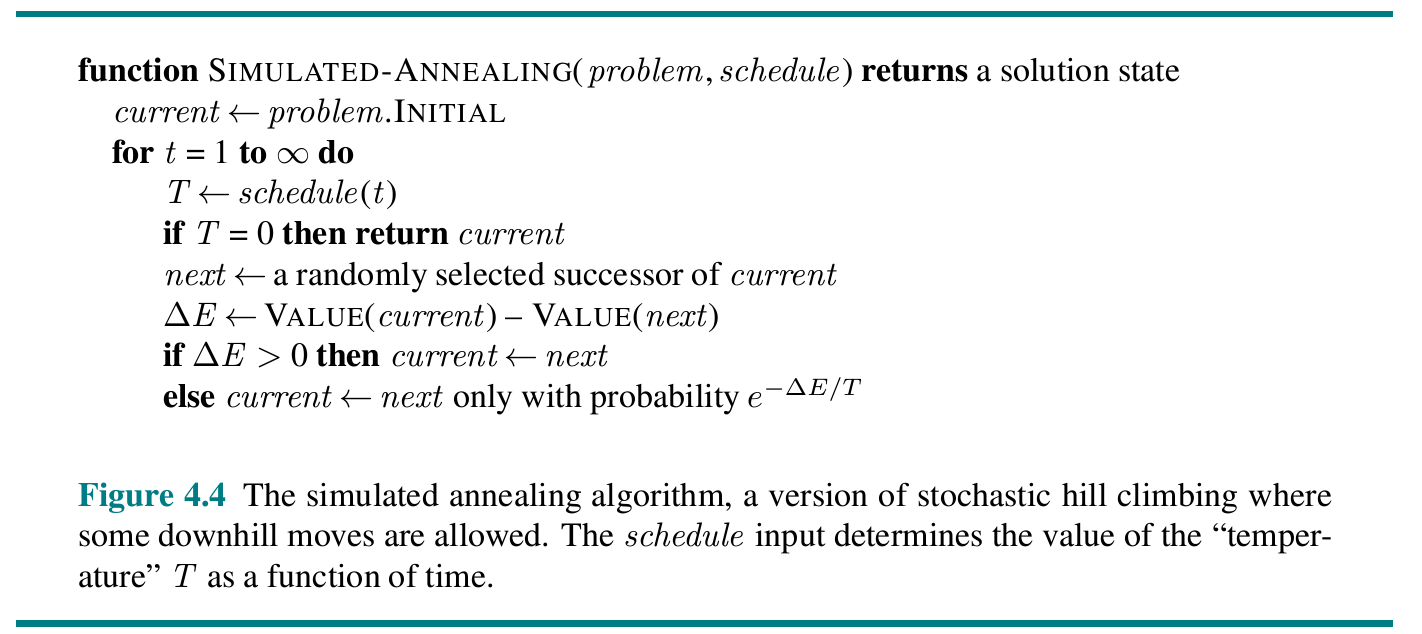
\includegraphics[scale=0.5]{./img/RecorridoSimulado}
\end{figure}


\end{frame} 


%%%%%%%%%%%%%%%%%%%%%%%%%%%%%%%%
\begin{frame} [fragile ]\frametitle{Recorrido Simulado en Python 1/2} \footnotesize
\begin{minted}[fontsize=\footnotesize]{python}

def simulated_annealing(problem, max_iterations=10000000):
    current_state = problem.state
    current_cost  = problem.calculate_cost(current_state)
    debug(f"current_state, {current_state}: {current_cost}")
    
    current_temperature = max_iterations

    while (not problem.is_goal_state()) and (current_temperature > 0):
        neighbors = problem.get_neighbors()
        debug(f"\t Neighbors:, {neighbors}")

        next_state = random.choice(neighbors)
        next_cost = problem.calculate_cost(next_state)  # Calculando el costo del próximo estado
        debug(f"\t\t next_state  {next_state} ({next_cost})")

        

\end{minted}

\end{frame} 
%%%%%%%%%%%%%%%%%%%%%%%%%%%%%%%%
\begin{frame} [fragile ]\frametitle{Recorrido Simulado en Python 2/2 } \footnotesize
\begin{minted}[fontsize=\tiny]{python}
        diff_cost = next_cost - current_cost       
        move =  False
        if (diff_cost <= 0):
            move = True
        else:
            boltz = math.exp(-float(diff_cost) / current_temperature)
            randomvalue = random.random()
            debug(f"\t\t diff_cost  {diff_cost}")
            debug(f"\t\t randomvalue  {randomvalue}, boltz {boltz}")
            if  randomvalue <= boltz:
                move = True
        if move:
            problem.state = next_state
            current_state = next_state
            current_cost = next_cost
            debug(f"current_state, {problem.state}: {current_cost}")

        current_temperature-=1
    
    if (problem.is_goal_state()):
        print (f"Solución encontrada en: {current_temperature}/{max_iterations}")
    
    return current_state

\end{minted}

\end{frame} 

%%%%%%%%%%%%%%%%%%%%%%%%%%%%%%%%
\begin{frame} \frametitle{ Puzzle 8: Energía, Recorrido Simulado} \small

\begin{figure}
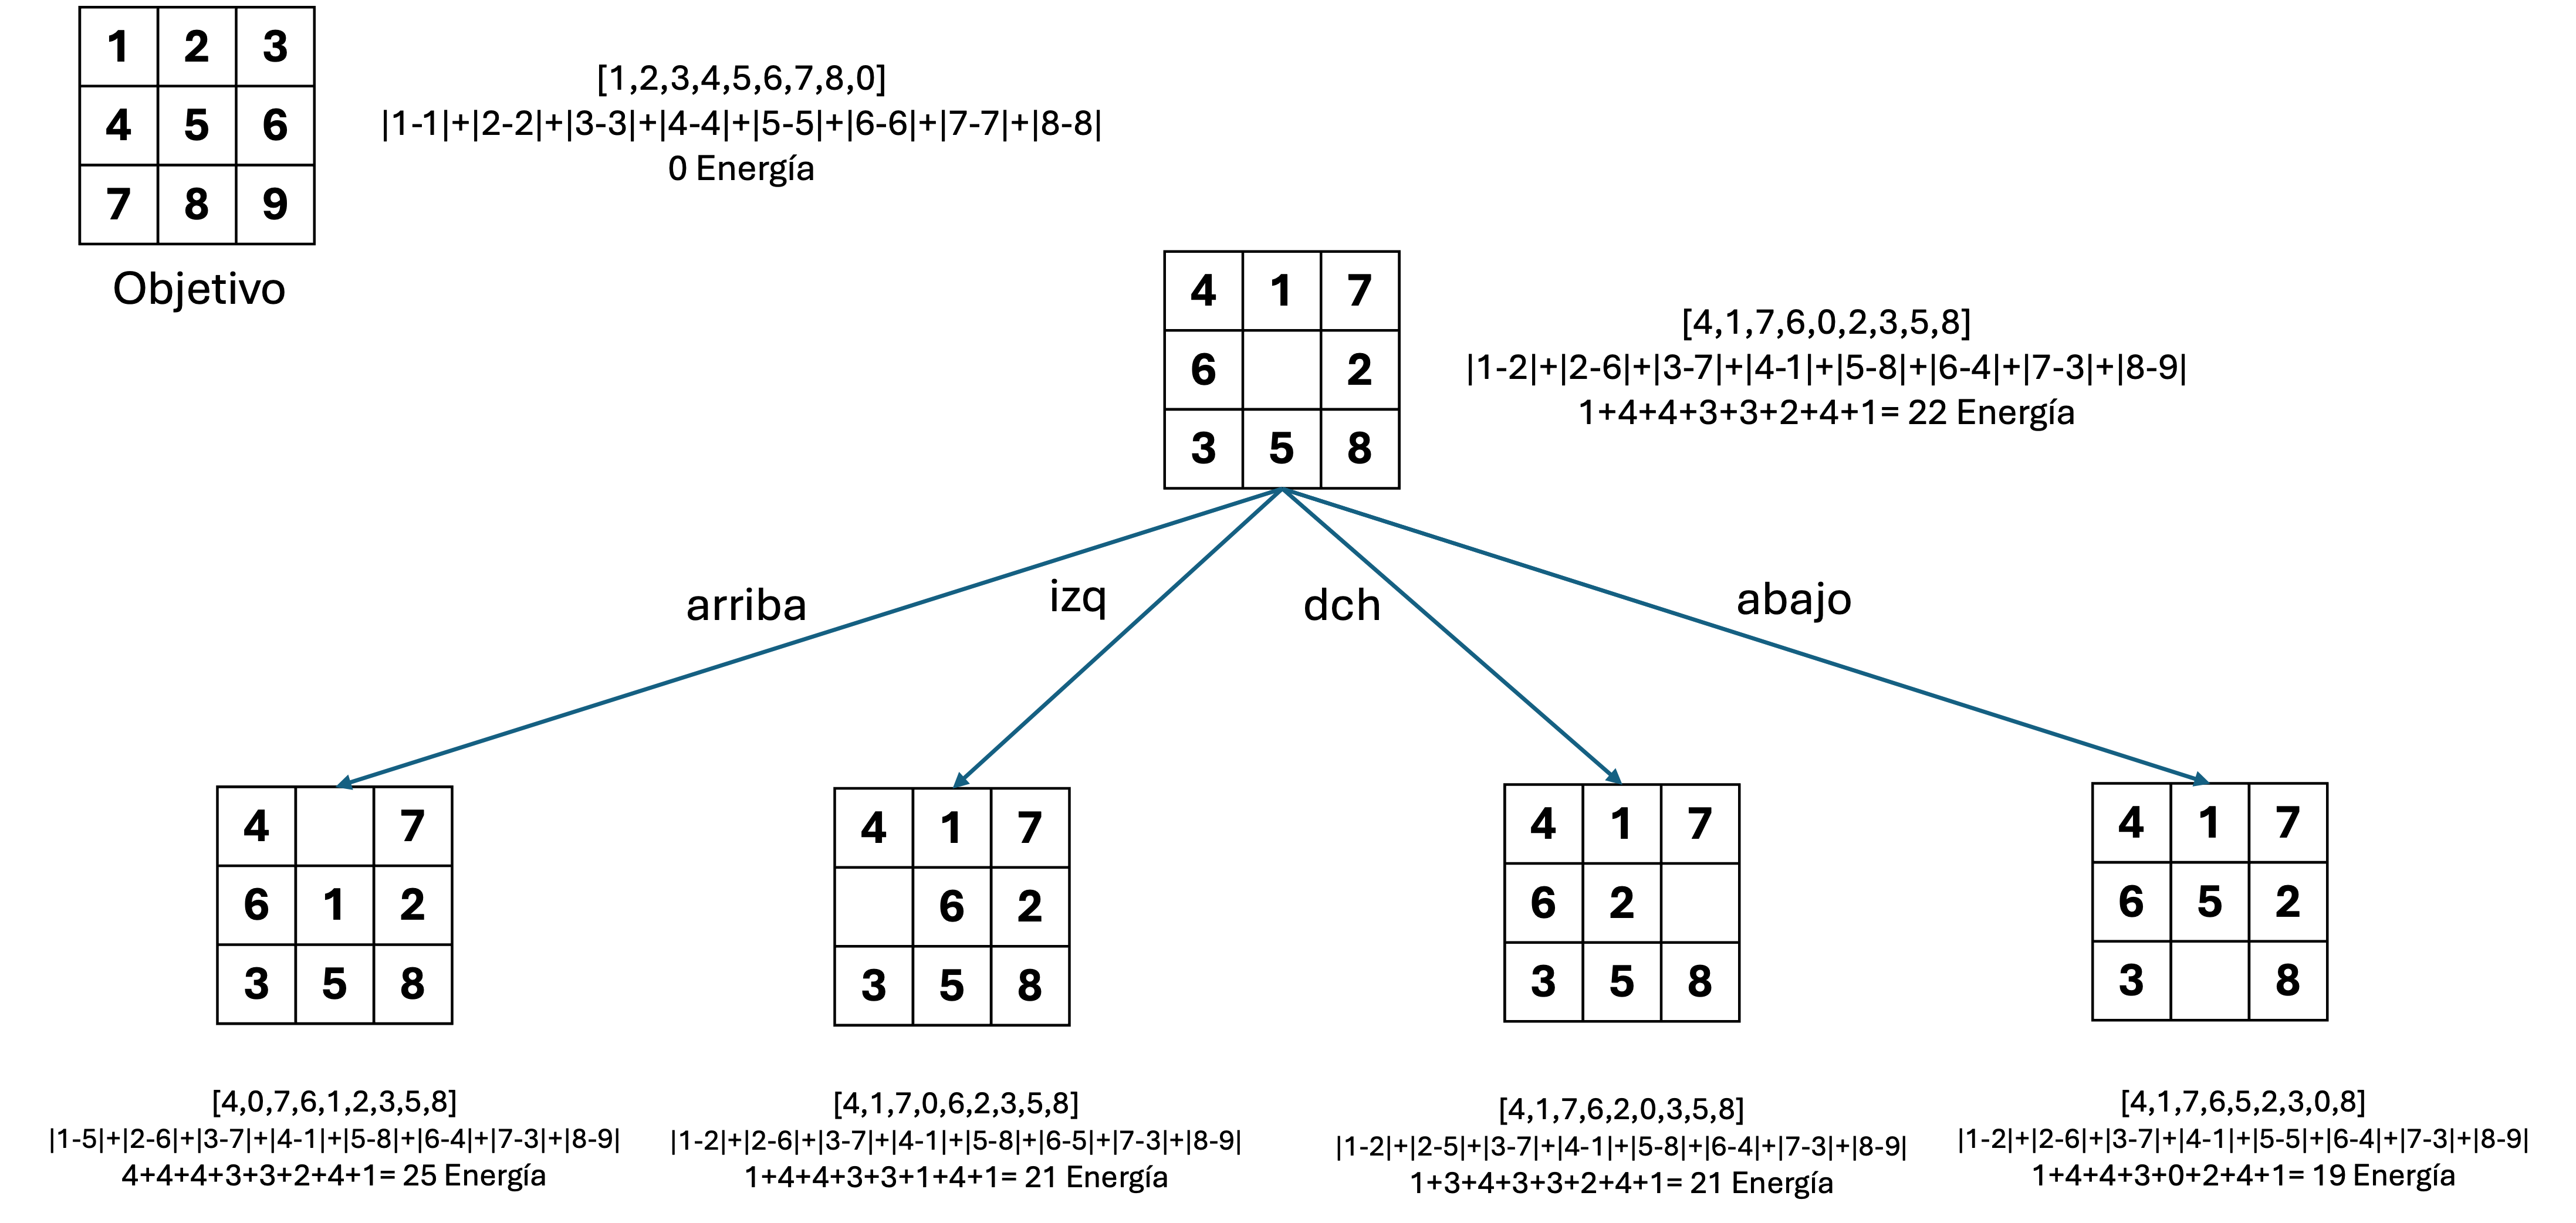
\includegraphics[scale=0.35]{./img/Puzzle8Energia}
\end{figure}


\end{frame} 

%%%%%%%%%%%%%%%%%%%%%%%%%%%%%%%%
\begin{frame} [fragile ]\frametitle{Recorrido Simulado en Python 2/2 } \footnotesize
\begin{minted}[fontsize=\tiny]{python}
        diff_cost = next_cost - current_cost       
        move =  False
        if (diff_cost <= 0):
            move = True
        else:
            boltz = math.exp(-float(diff_cost) / current_temperature)
            randomvalue = random.random()
            debug(f"\t\t diff_cost  {diff_cost}")
            debug(f"\t\t randomvalue  {randomvalue}, boltz {boltz}")
            if  randomvalue <= boltz:
                move = True
\end{minted}

 diff\_cost = next\_cost - current\_cost\\ 
 \hspace{1cm} = 19 - 22 = -3\\
 \hspace{1cm} = 21 - 22 = -1\\
 \hspace{1cm} = 25 - 22 = 3

 boltz = math.exp(-float(diff\_cost) / current\_temperature)\\
 current\_temperature= 40 -> $e^{-3/40}$ = 0.9277 = 92.77\%
\end{frame} 

%%%%%%%%%%%%%%%%%%%%%%%%%%%%%%%%

\begin{chapter}[images/etsiinformatica4.png]{uicblue}{Búsqueda local\\
Algoritmos Genéticos}
\end{chapter}
\subsection{Algoritmos Genéticos}
%%%%%%%%%%%%%%%%%%%%%%%%%%%%%%%%
%%%%%%%%%%%%%%%%%%%%%%%%%%%%%%%%

%%%%%%%%%%%%%%%%%%%%%%%%%%%%%%%%

\begin{frame} \frametitle{ Esquema General} \small

\begin{figure}
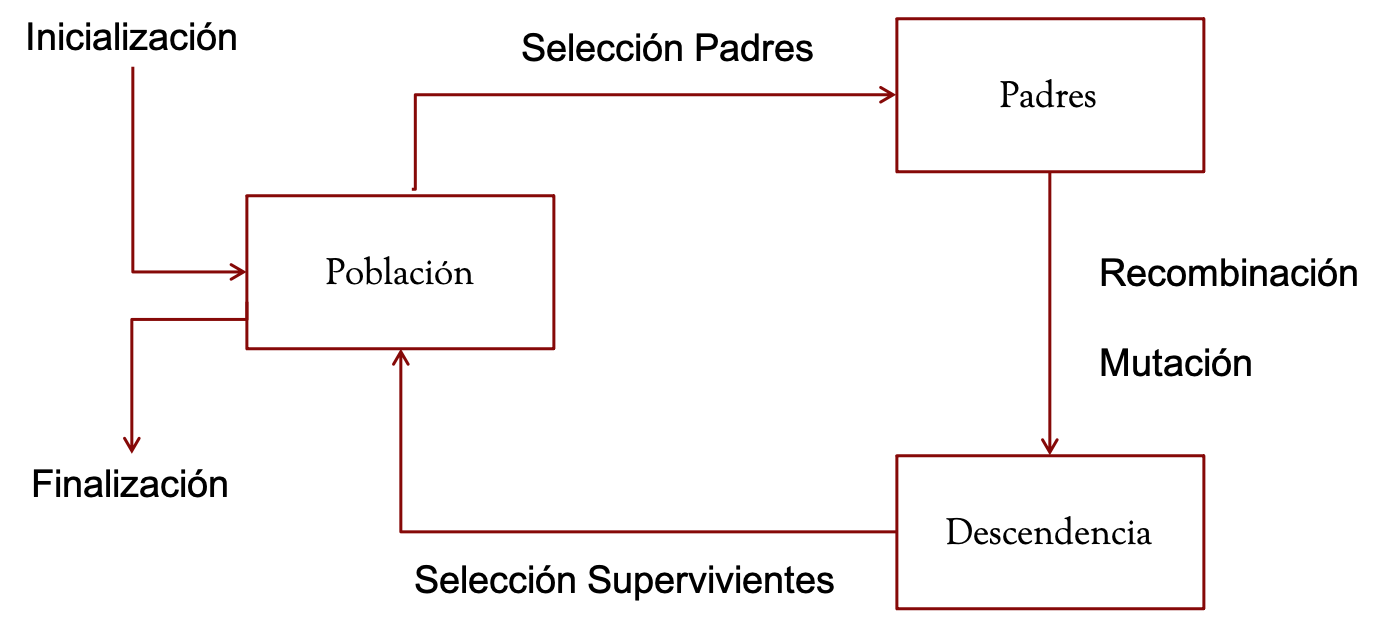
\includegraphics[scale=0.5]{./img/AlgoritmoGeneticoEsquema}
\end{figure}


\end{frame} 

%%%%%%%%%%%%%%%%%%%%%%%%%%%%%%%%

\begin{frame} \frametitle{ Esquema General} \small

\begin{figure}
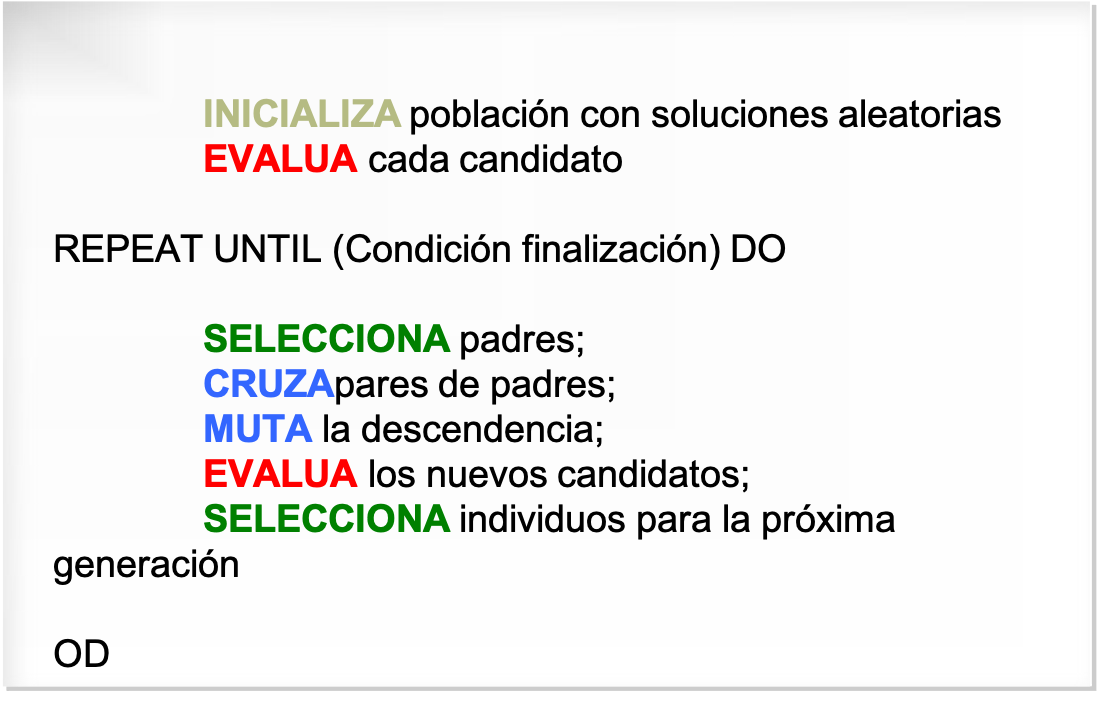
\includegraphics[scale=0.5]{./img/AlgoritmoGeneticoEsquema2}
\end{figure}


\end{frame} 


%%%%%%%%%%%%%%%%%%%%%%%%%%%%%%%%

\begin{frame} \frametitle{ Definiciones} \small

\begin{description}
\item[Población]: Comenzamos con un conjunto de k estados generados de forma aleatoria. 
\item[Función idoneidad]: Cada estado se tasa con una función de evaluación. Valores más altos para los mejores valores.
\item[Cruce] : Seleccionamos dos pares de forma aleatoria para la reproducción, según con las probabilidades. 
Además se selecciona aleatoriamente un punto de cruce.
\item[Mutación] : Finalmente se realiza una mutación aleatoria con una probabilidad independiente. 
	
\end{description}

\end{frame} 

%%%%%%%%%%%%%%%%%%%%%%%%%%%%%%%%

\begin{frame} \frametitle{ Algoritmo pseudocódigo} \small

\begin{figure}
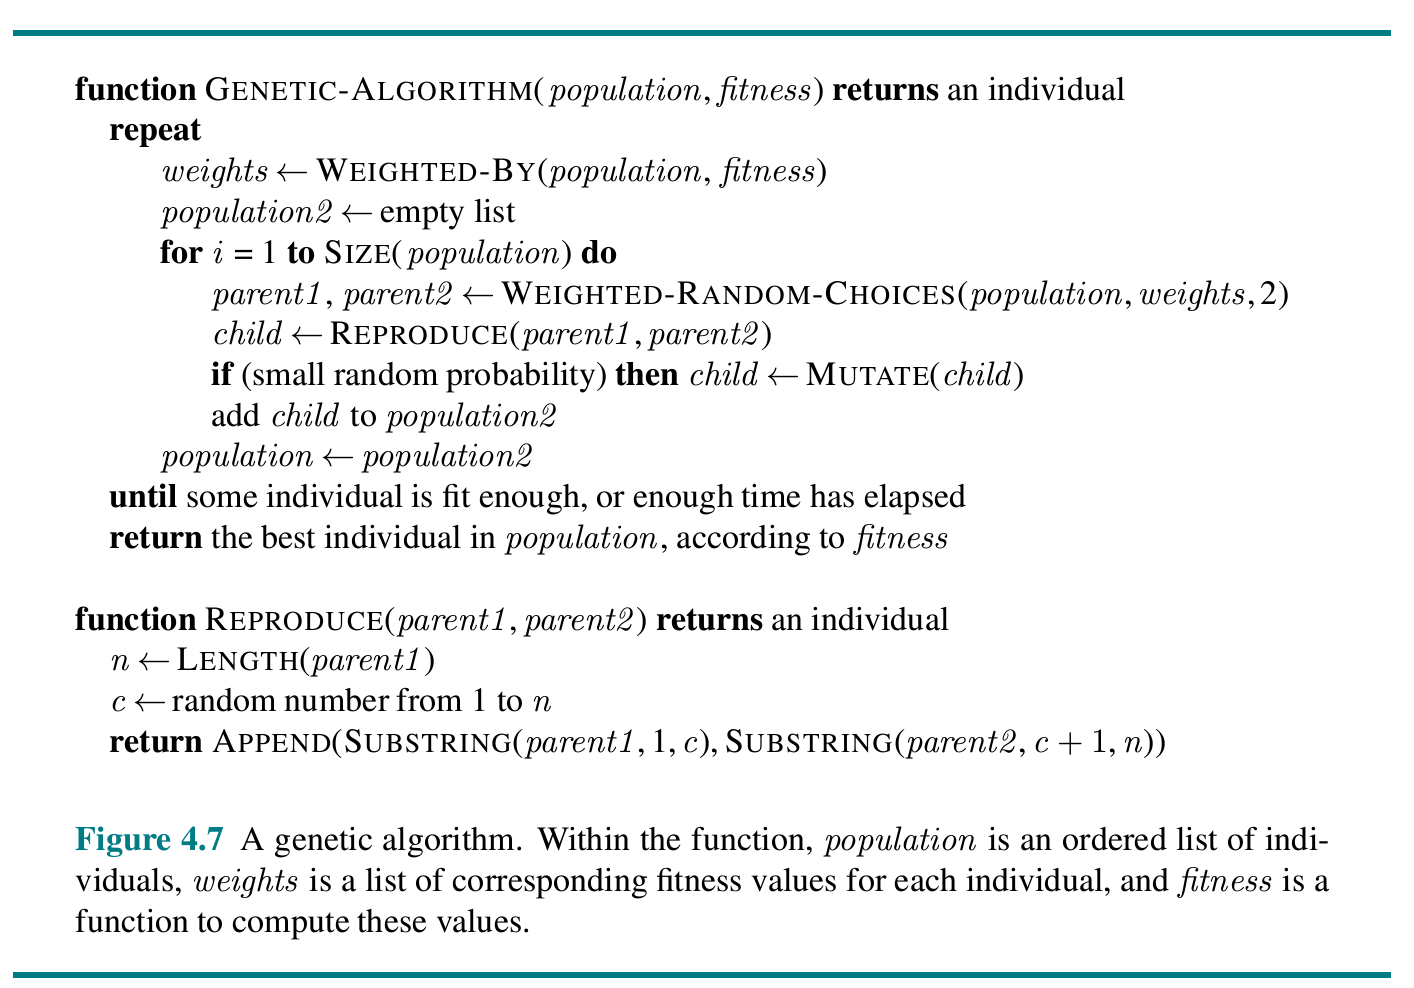
\includegraphics[scale=0.35]{./img/AlgoritmoGenetico}
\end{figure}


\end{frame} 



%%%%%%%%%%%%%%%%%%%%%%%%%%%%%%%%

\begin{frame} \frametitle{ Ejemplo 8 Reinas - Genéticos} \tiny

\begin{itemize}
\item El objetivo del problema es establecer 8 reinas en un tablero de forma que no se ataquen entre sí. 
\item Evitar Misma fila, columna o diagonal.
\end{itemize}

\begin{description}
\item[Estado] : Cualquier representación de 8 reinas en el tablero.
\item[Estado Inicial] : Tablero con 8 reinas
\item[Acciones] : Mover una reina a una casilla vacía de una columna
\item[Modelo Transición] : Devuelve tablero con una reina añadida en una casilla determinada.
\item[Test Objetivo] : 8 reinas en el tablero que no se ataquen entre sí.
\item[Función Heurística] : Número de pares de reinas que se atacan (MIN) 
\end{description}




\begin{figure}
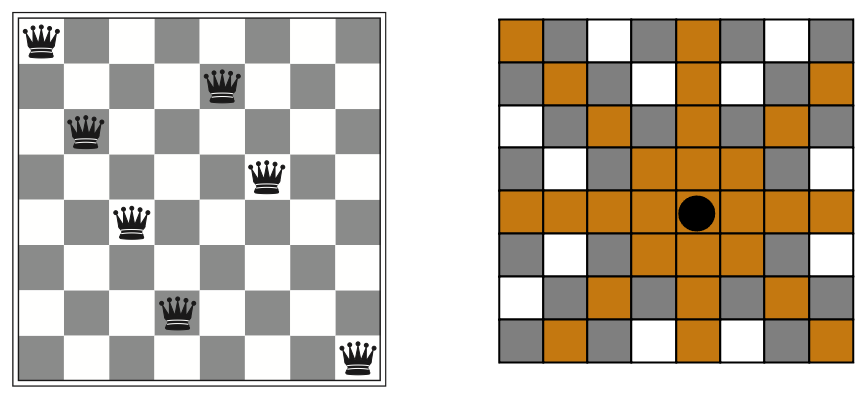
\includegraphics[scale=0.45]{./img/8Reinas}
\end{figure}


\end{frame} 


%%%%%%%%%%%%%%%%%%%%%%%%%%%%%%%%

\begin{frame} \frametitle{ Ejemplo 8 Reinas - Genéticos} \small

\textbf{Representación Problema}

\begin{figure}
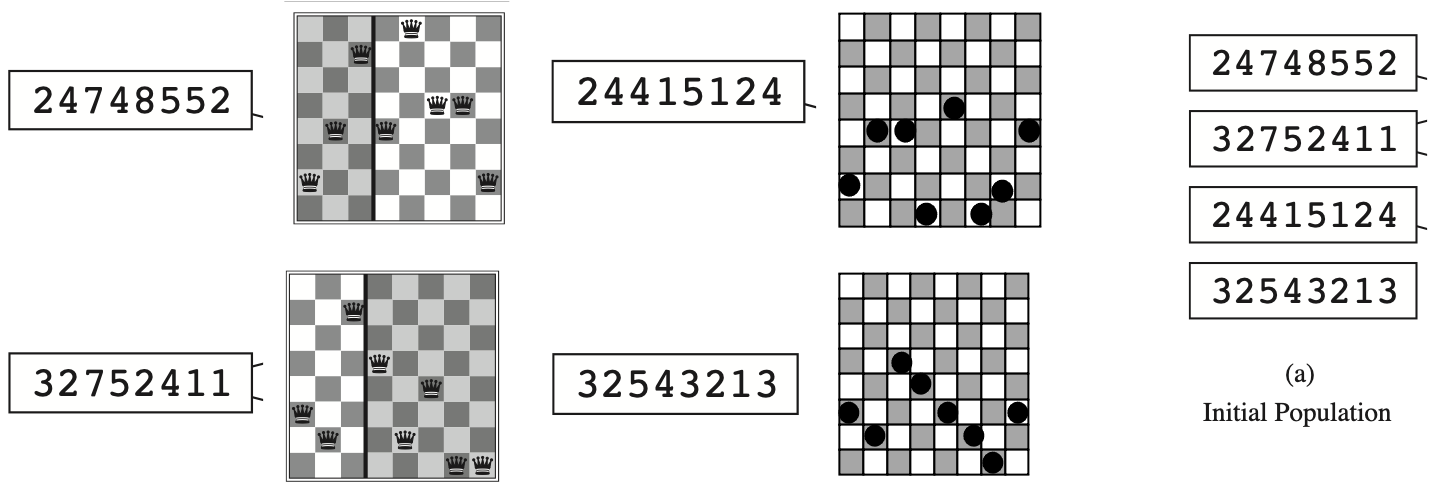
\includegraphics[scale=0.4]{./img/8ReinasGeneticos1}
\end{figure}

\end{frame} 

%%%%%%%%%%%%%%%%%%%%%%%%%%%%%%%%

\begin{frame} \frametitle{ Ejemplo 8 Reinas - Genéticos} \small

\textbf{Función Evaluación}:Número de pares de reinas que ``no atacan''

\begin{figure}
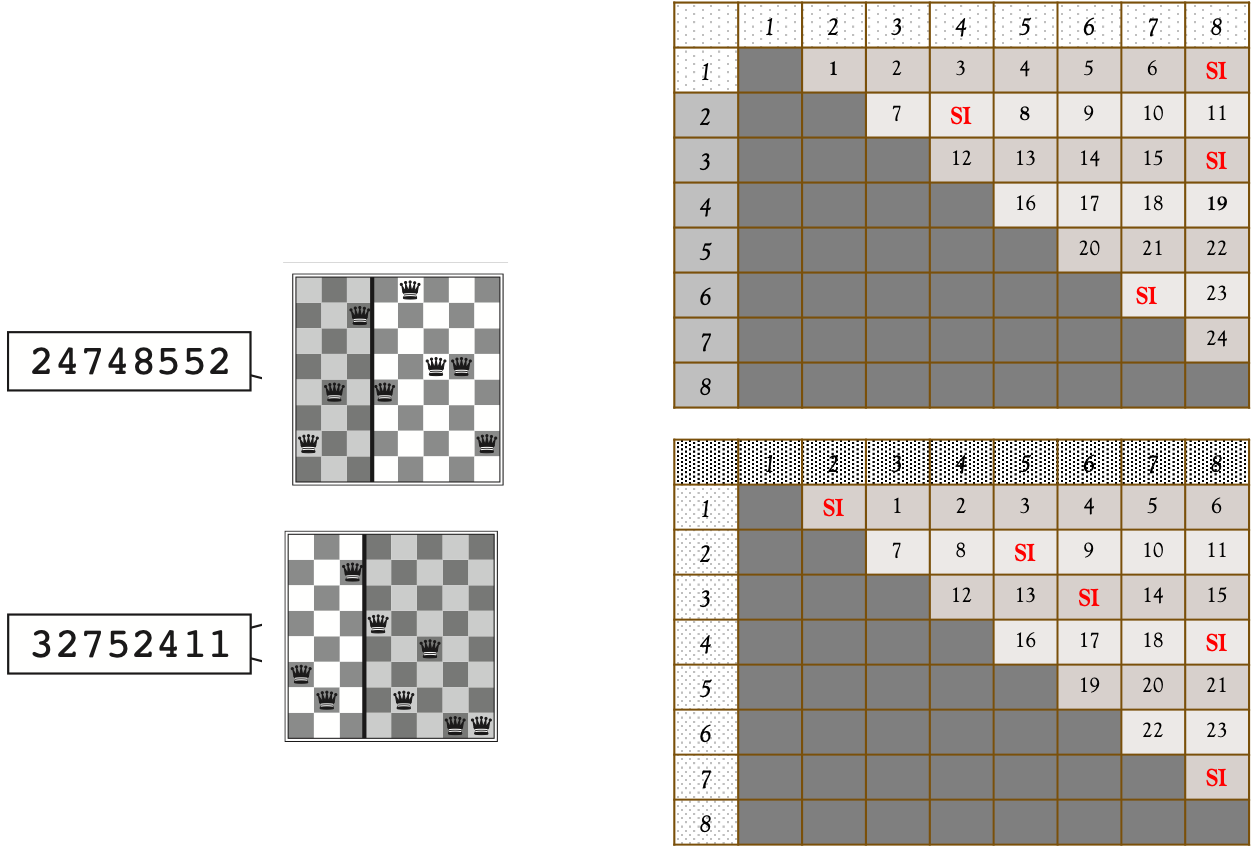
\includegraphics[scale=0.37]{./img/8ReinasGeneticos2}
\end{figure}

\end{frame} 

%%%%%%%%%%%%%%%%%%%%%%%%%%%%%%%%

\begin{frame} \frametitle{ Ejemplo 8 Reinas - Genéticos} \small

\textbf{Función Evaluación} 

\begin{figure}
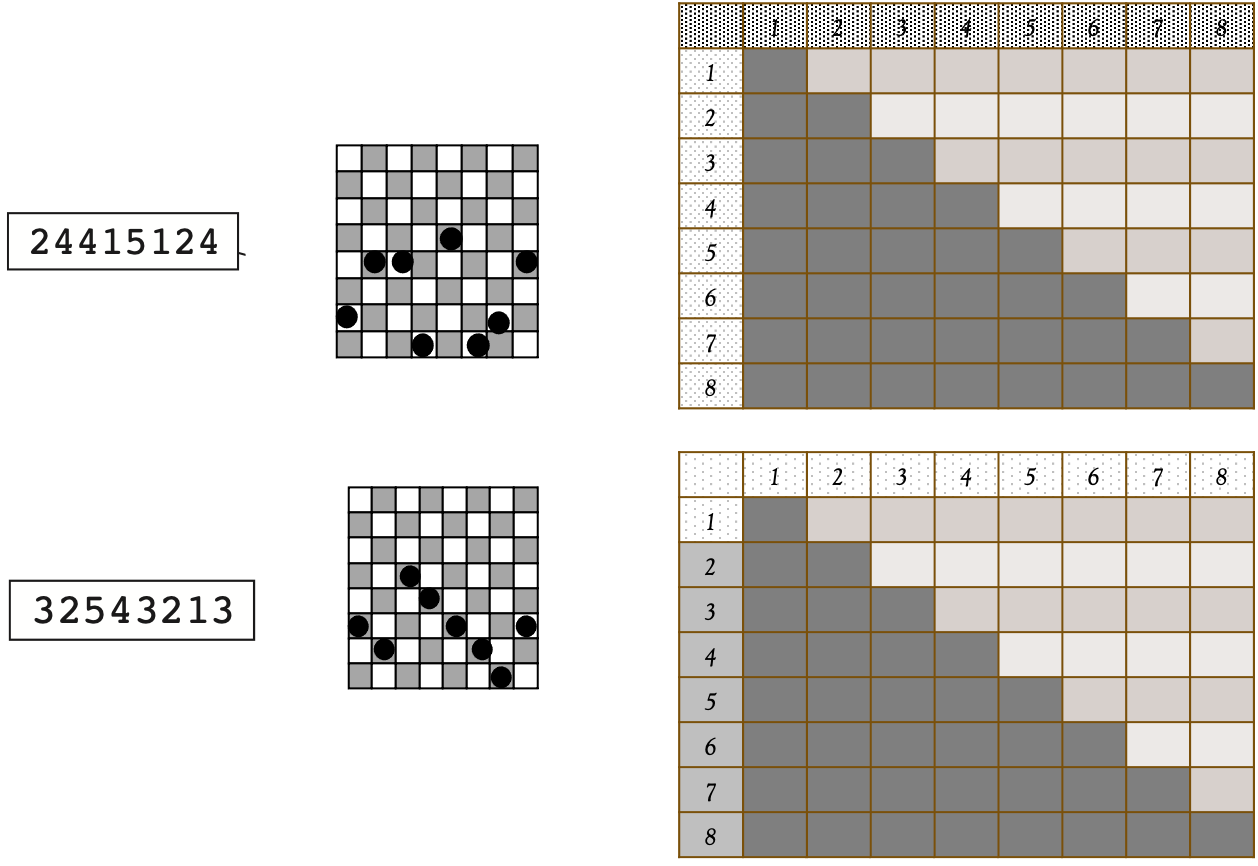
\includegraphics[scale=0.37]{./img/8ReinasGeneticos3}
\end{figure}

\end{frame} 

%%%%%%%%%%%%%%%%%%%%%%%%%%%%%%%%

\begin{frame} \frametitle{ Ejemplo 8 Reinas - Genéticos} \small

\textbf{Evaluación y Selección} 

\begin{figure}
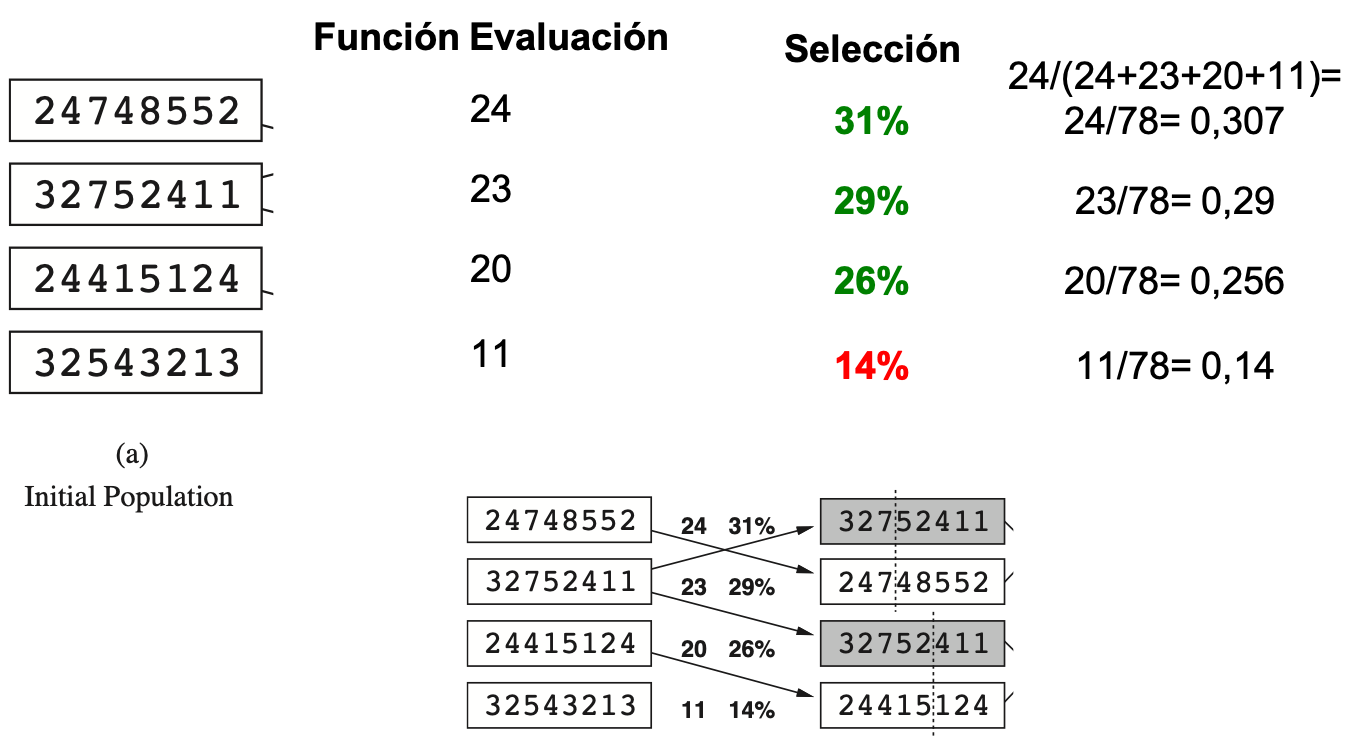
\includegraphics[scale=0.37]{./img/8ReinasGeneticos4}
\end{figure}

\end{frame} 


%%%%%%%%%%%%%%%%%%%%%%%%%%%%%%%%

\begin{frame} \frametitle{ Ejemplo 8 Reinas - Genéticos} \small

\textbf{Cruce} 

\begin{enumerate}
\item Selecciona un punto de cruce aleatorio
\item Copia la primera parte de un padre al hijo
\item Copia la segunda parte de otro padre al hijo
\end{enumerate}


\begin{figure}
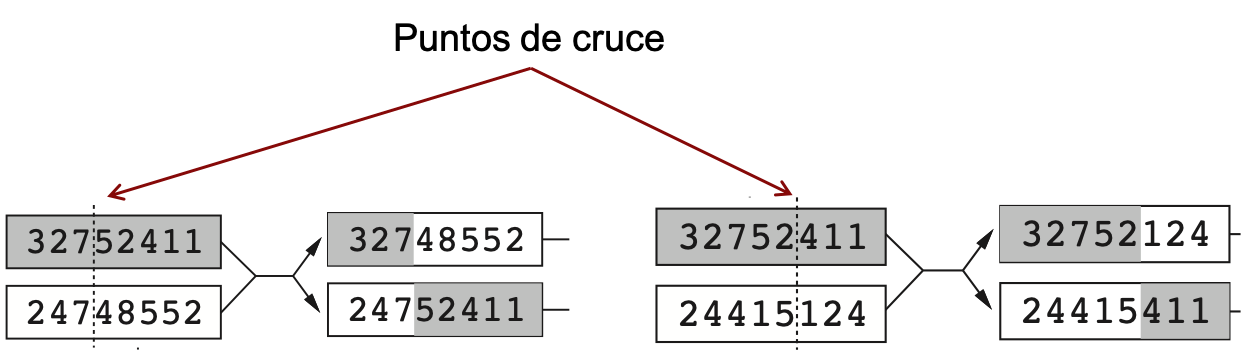
\includegraphics[scale=0.4]{./img/8ReinasGeneticos5}
\end{figure}

\end{frame} 

%%%%%%%%%%%%%%%%%%%%%%%%%%%%%%%%

\begin{frame} \frametitle{ Ejemplo 8 Reinas - Genéticos} \small

\textbf{Mutación} 

\begin{itemize}
\item Posibles Operaciones:
\begin{itemize}
\item Intercambia dos valores de posición
\item Cambia el valor aleatorio de una posición
\end{itemize}

\item Puede resultar una configuración no válida
\end{itemize}



\begin{figure}
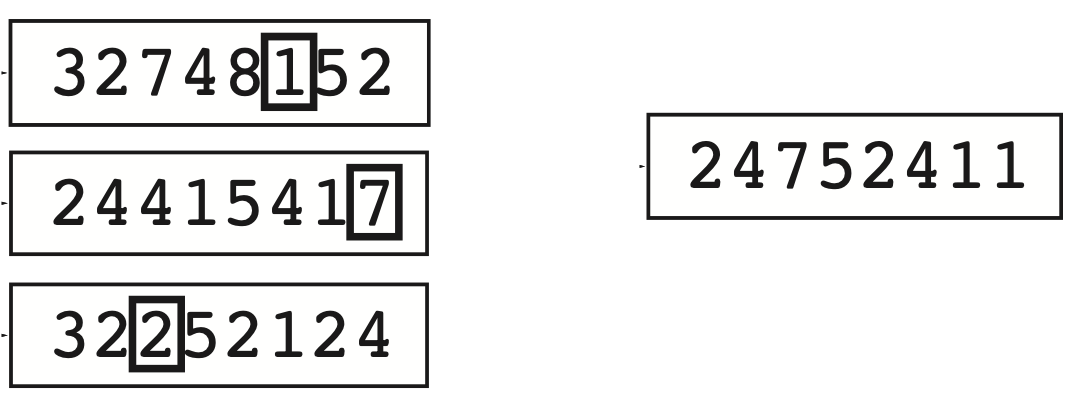
\includegraphics[scale=0.4]{./img/8ReinasGeneticos6}
\end{figure}

\end{frame} 

%%%%%%%%%%%%%%%%%%%%%%%%%%%%%%%%

\begin{frame} \frametitle{ Ejemplo 8 Reinas - Genéticos} \small


\begin{figure}
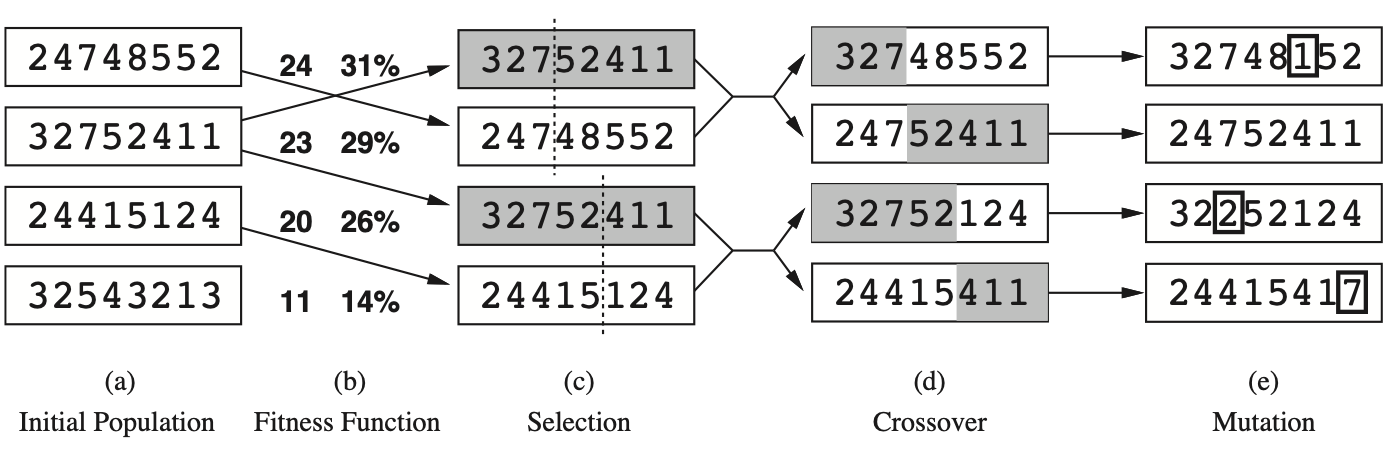
\includegraphics[scale=0.45]{./img/8ReinasGeneticos7}
\end{figure}

\end{frame} 



%%%%%%%%%%%%%%%%%%%%%%%%%%%%%%%%
%\begin{frame} [fragile ]\frametitle{Puzzle 8 - Heurístico} \footnotesize
%\begin{minted}[fontsize=\small]{python}

%initial_state = '1'
%goal_state = '8'
%problem = ProblemGrafo(initial_state, goal_state)
%solution_node = depth_first_search(problem)
%\end{minted}

%\end{frame} 







%%%%%%%%%%%%%%%%%%%%%%%%%%%%%%%%
%\begin{frame}  \small  
%\end{frame} 


%%%%%%%%%%%%%%%%%%%%%%%%%%%%%%%%
%\begin{frame}  \small  
%\end{frame} 


%%%%%%%%%%%%%%%%%%%%%%%%%%%%%%%%
%\begin{frame}  \small  
%\end{frame} 

%%%%%%%%%%%%%%%%%%%%%%%%%%%%%%%%
%%%%%%%%%%%%%%%%%%%%%%%%%%%%%%%%

%%%%%%%%%%%%%%%%%%%%%%%%%%%%%%%%
%%%%%%%%%%%%%%%%%%%%%%%%%%%%%%%%
   
\backmatter


\end{document}